% Definition der Klasse des Dokumentes
\documentclass[12pt, a4paper]{article}

% Standardpakete für deutsche Sprache
\usepackage[utf8]{inputenc}
\usepackage[ngerman]{babel}

\usepackage{csquotes}

% Volle Seite nutzen
\usepackage{fullpage} 
\headsep 1cm
\parindent 0cm

\usepackage{float}

% einige Pakete für Mathematische Darstellung
\usepackage{amssymb, amstext, amsmath}
\usepackage{fancyhdr}

\usepackage{booktabs}

\usepackage{listings}

% ein Paket für die Zählung von Seiten
\usepackage{count1to}
\usepackage{lastpage} 

%Paket für Aufzählungsbuchstaben
\usepackage{enumitem}

\usepackage{setspace}
\makeatletter
\newcommand{\MSonehalfspacing}{%
	\setstretch{1.44}%  default
	\ifcase \@ptsize \relax % 10pt
	\setstretch {1.448}%
	\or % 11pt
	\setstretch {1.399}%
	\or % 12pt
	\setstretch {1.433}%
	\fi
}
\newcommand{\MSdoublespacing}{%
	\setstretch {1.92}%  default
	\ifcase \@ptsize \relax % 10pt
	\setstretch {1.936}%
	\or % 11pt
	\setstretch {1.866}%
	\or % 12pt
	\setstretch {1.902}%
	\fi
}
\makeatother
\MSonehalfspacing

%\usepackage{csquotes}

% Kopfzeile und Fußzeile
\lhead{Laserprojekt}
\chead{}
\rhead{\today}
\lfoot{Jan Pohlmeyer \& Janneke Simmering}
\rfoot{\thepage\ von \pageref{LastPage}}
\cfoot{}

% Wird zur Einbindung von Bildern benötigt
\usepackage{graphicx}
\graphicspath{{pictures/}}
% Einbinden des Literaturverzeichnisses
%\usepackage[backend=bibtex,style=numeric-comp]{biblatex}
%\bibliography{literatur.bib}
%\addbibresource{literatur.bib}

% Wird zum Einbinden von LaTeX Code benötigt
\usepackage{color}
\usepackage{showexpl}

\renewcommand{\footrulewidth}{0.4pt}
\pagestyle{fancy}

% Konfiguration des Deckblatts
\begin{titlepage}
\title{\textbf{Angewandte Robotik \\ Laserprojekt}}
\author{Jan Pohlmeyer \& Janneke Simmering}
\date{\today}
\end{titlepage}

\begin{document}
% Einfügen des Deckblatts
\clearpage
\maketitle
\thispagestyle{empty}


\tableofcontents
\thispagestyle{empty}

\newpage

\setcounter{page}{1}

\section{Aufgabe 1 -- Hindernisvermeidung (Jan)}

Damit ein mobiler Roboter eine Karte von einem Raum aufnehmen kann muss er sich natürlich durch den Raum bewegen können um alle Ecken zu erreichen. Dabei ist es unumgänglich eine Strategie zu implementieren mithilfe derer der Roboter durch den Raum fährt ohne mit Hindernissen und Wänden zu kollidieren.
Da der Laserscanner eine Reichweite von etwa 8 Metern hat muss der Raum nicht unbedingt systematisch abgefahren werden. Es reicht, wenn der Roboter alle Ecken des Raumes mit dem Laserscanner mindestens einmal aufnehmen kann. In Abbildung~\ref{fig:kartonRaumLabor} ist Testbereich zu sehen, der im Labor mithilfe von Pappkartons aufgebaut wurde. Der Roboter soll zum Beispiel in diesem Bereich eine Karte aufnehmen können.

\begin{figure}[H]
	\centering
	\includegraphics[width=10cm]{kartonRaumLabor}
	\caption{Ein mithilfe von Kartons errichteter Testbereich für das Aufnehmen einer Karte.}
	\label{fig:kartonRaumLabor}
\end{figure}

Die Strategie, die wir zuerst implementiert haben, hat versucht leicht vom nächsten Hindernis weg zu lenken. Es wird der Scanpunkt mit dem minimalen Abstand bestimmt und wenn dieser eher auf der rechten Seite des Roboters liegt wird leicht nach links gesteuert, bzw. falls das nächste Hindernis sich eher links befindet, wird leicht rechts gesteuert. Wenn der minimale Abstand aber über einem Threshold von 1,2 Metern liegt, fährt der Roboter einfach weiter geradeaus.
Ein Problem mit diesem Ansatz trat auf, falls der Roboter in eine Sackgasse gefahren war und dann schräg vor einer der Ecken stand.
Dies haben wir zunächst versucht durch eine Sackgassenerkennung zu beheben, die auf ein lokales Maximum geradeaus vor dem Roboter prüft.
Leider hat dieser Lösungsansatz nicht so gut geklappt und häufig wurde der Autostop des Roboters ausgelöst. Da wir ein weiteres Problem dieses Ansatzes mit Löchern in den Wänden (zwischen den Kartons) sahen, haben wir uns dann entschieden den Ansatz zu wechseln.

Der neue Ansatz soll nun zum Einen das Problem der Sackgassen lösen und auch mit Spalten zwischen den Wänden klarkommen. Dazu werden die Scanpunkte zunächst in 3 gleich große Bereiche aufgeteilt. Der erste Bereich sind die Punkte, die eher zur rechten Seite des Roboters liegen. Der zweite Bereich sind die Punkte, die geradeaus vor dem Roboter liegen und der dritte Bereich sind schließlich die Punkte, die links vom Roboter liegen. In jedem der Bereiche werden nun die Scanpunkte gezählt, die einen bestimmten Distanzthreshold unterschreiten. Zunächst haben wir den Threshold auf 1,2m gesetzt, damit wir mit aktivem Autostop testen konnten.
Auch für die Anzahl Scanpunkte, ab dem ein Bereich als ''nah'' gilt wurde ein Threshold auf 5 Stück festgelegt. Dies verhindert, dass durch Ausreißerpunkte eine Hindernisvermeidung angestoßen wird und schlägt trotzdem direkt an, falls ein echtes Hindernis im Weg auftauchen sollte.
Falls sich im vorderen Bereich nun weniger Scanpunkte finden als dieser Threshold, dann wird einfach weiter der alte Ansatz verfolgt. Wenn sich allerdings im vorderen Bereich ein Hindernis befindet, dann verhält der Roboter sich anders. Zunächst vergleicht er die Anzahl Scanpunkte auf der linken und der rechten Seite deren Distanz unter dem Threshold ist. Falls links weniger Punkte als rechts sind fährt er eine scharfe links Kurve, falls rechts weniger Punkte sind eine scharfe rechts Kurve. Falls aber auf beiden Seiten ungefähr gleich viele Punkte sind und die Punkteanzahl den Threshold von 5 Punkten überschreitet geht er von einer Sackgasse aus und versucht sich umzudrehen indem er auf der Stelle dreht. Falls auf beiden Seiten ungefähr gleich viel Platz scheint fährt er einfach eine scharfe rechts Kurve.
Dieser Ansatz funktioniert ziemlich gut und wir konnten den Autostop deaktivieren um zu testen wie weit wir den Distanzthreshold verringern können. Letztendlich haben wir den Threshold auf 0,7 Meter runtergesetzt. Der Roboter vermeidet Hindernisse nun sehr zuverlässig ohne aber Ecken eines Raumes komplett auszulassen. Er schafft es sogar selbstständig durch die Labortür auf den Flur.

\section{Aufgabe 2 -- Aufnehmen einer Karte}

Im zweiten Teil des Projekts ging es darum den Pioneer-Roboter mithilfe des SICK-Laserscanners eine Karte aufbauen zu lassen. Das benutzte Verfahren basiert auf dem Paper "Keeping Track of Position and Orientation of Moving Indoor Systems by Correlation of Range-Finder Scans" von Gerhard Weiß et al.. Der verwendete Laserscanner hat einen Öffnungswinkel von 180 Grad, während der Laserscanner im Paper einen Öffnungswinkel von 360 Grad aufweist. Im Folgenden berichten wir schrittweise von unserem Implementationsweg.

\section{Winkelhistogramme (Janneke)}

erster naiver ansatz (ohne rauschen)

berechne winkel der geraden wenn man einen scanpunkt mit dem nächsten verbindet (angle=atan2(y1-y2,x1-x2))
umrechnen in grad
einteilen in bins im histogramm (angle+180)/(360/BINCOUNT)
zählen in den entsprechenden bins

darstellen im histogramm fenster mit kreisen

(winkelhistogramLaserOhneRauschen)

\section{Korrelation der Winkelhistogramme}

berechnen der korrelation zwischen dem aktuellen winkelhistogramm und dem vorherigen winkelhistogram

korrelationsformel: blub

einteilen der korrlationswerte in bins

skalieren der grafischen ausgabe

\section{Rotationskorrektur}

zunächst nur mit odometriedaten korrigieren -> klappt nicht: globalen offset mit speichern und erhöhen weil in jedem schritt nur relativer offset berechnet wird

dann finden des lokalen maximums der korrelation mithilfe der odometriedaten als ausgangspunkt für die suche

erster ansatz: gleichzeitig nach links und nach rechts vom odometriepunkt suchen, bis ein wert gefunden wurde, der mindestens 50\% des maximalen korrelationswert hat. später hochgesetzt auf 2/3 des maximalen korrelationswert hochgesetzt -> idee: kein lokales maximum im rauschen finden sondern klares maximum finden

funktioniert manchmal nicht ganz so gut, manchmal maxima nicht gefunden, da dies zu klein ist (spaeter durch rauschen vermutlich noch schlimmer)..

neuer ansatz: in 15 grad um den odometriepunkt den maximalen punkt in der korrelation suchen -> besser

entsprechend dem lokal maximalen bin der korrelation den scan rotieren und die rotation auf den globalen offset aufaddieren und den scan in die karte eintragen

\subsection{Ausrichten der Wände auf die Hauptachsen (Janneke)}

Bisher haben wir die Translation der Karte um andere Bewegungen des Roboters auszugleichen noch gar nicht beachtet. Hierfür können X- und Y-Histogramme verwendet werden. Um ein X- bzw. Y-Histogramm zu erstellen muss allerdings der Scan hauptachsenaligned sein. Das heißt, dass die Wände bzw. geraden Linien im Scan parallel zur X- oder Y-Achse liegen müssen.

Dies könnte man nur für die Erstellung der Histogramme in jedem Schritt für jeden Scan einzeln machen, wir haben uns jedoch anders als im Paper dafür entschieden unseren initialen Scan so auszurichten da dann jeder weitere Scan durch die Rotationskorrektur auf den ersten Scan ausgerichtet wird und damit automatisch auch auf die Hauptachsen ausgerichtet wird.

Also suchen wir das Maximum im Winkelhistogramm des ersten Scans, welches der prominentesten Wand entsprechen würde. Dann rotieren wir den Scan so, dass der berechnete Winkel auf die Null im Histogramm verschoben wird. Diese Rotation setzen wir nun als initialen Rotationsoffset. Der rotierte Scan wird dann in die Karte eingezeichnet, sodass unsere resultierende Karte auch direkt hauptachsenaligned ist.

\begin{figure}
	\centering
	\includegraphics[width=11cm]{hauptachsenalignedMap}
	\caption{Eine Karte die auf die Hauptachsen ausgerichtet wurde.}
	\label{fig:Hauptachsenaligned}
\end{figure}

Abbildung~\ref{fig:Hauptachsenaligned} zeigt eine Karte in die der initiale, auf die Hauptachsen ausgerichtete, Scan eingezeichnet ist.

\subsection{X- und Y-Histogramme (Jan)}

Nachdem der Scan auf die Hauptachsen ausgerichtet wurde kann ein X- und Y-Histogramm erstellt werden. Diese Histogramme stellen eine Statistik über die Anzahl der Punkte in X- bzw. Y-Richtung auf.
Dadurch, dass der Scan auf die Hauptachsen ausgerichtet wurde, fallen die X- bzw. Y-Koordinaten der Punkte auf einer Wand immer auf denselben X- bzw. Y-Wert. Es bildet sich nun für jede Wand ein Maximum in einem der beiden Histogramme. Wichtig, damit diese Methode funktioniert ist, dass die Wände gerade sind und sich an den Ecken 90 Grad Winkel befinden. Falls eine Wand nicht parallel zu einer der Hauptachsen liegt, verteilen sich die Punkte der Wand und bilden kein Maximum. Die Größe der im Histogramm abbildbaren Werte wird anhand der maximal messbaren Distanz in dem vorliegenden Raum angepasst. Diese muss sowohl in positiver Achsenrichtung, als auch in negativer Richtung aufgetragen werden können. In der Mitte der Histogramme befindet sich der Nullpunkt.

%TODO: grafik?

\subsection{Korrelation der X- und Y-Histogramme (Jan)}

Für die Korrelation der X- und Y-Histogramme haben wir denselben Ansatz wie auch schon für die Korrelation der Winkelhistogramme verfolgt. Das X- bzw Y-Histogramm des neuen Scans wird gegen das X- bzw. Y-Histogramm des alten Scans verschoben und eine X- bzw. Y-Korrelation wird für alle Verschiebungen berechnet. Am linken Rand der Korrelation befindet sich der Wert für eine Verschiebung um 0. Nach rechts ist dann eine positive Verschiebung aufgetragen. Die Verschiebung ist zyklisch geschlossen, deshalb ist eine große positive Verschiebung gleichbedeutend mit einer kleinen negativen Verschiebung.

\begin{figure}
	\centering
	\includegraphics[width=16cm]{XYhistogram}
	\caption{X- und Y-Histogramm einer Bewegung in Y-Richtung auf eine Wand zu. In blau ist das Histogramm des alten Scans eingetragen, in grün das Histogramm des neuen Scans und in rot die Korrelation der beiden Scans}
	\label{fig:xyhistogram}
\end{figure}

Abbildung~\ref{fig:xyhistogram} stellt die Histogramme und deren Korrelation bei einer Bewegung des Roboters in Y-Richtung auf eine Wand zu dar. Im X-Histogramm lässt sich deutlich erkennen, dass der Roboter sich parallel zu den Wänden bewegt. Die Maxima der neuen und alten Korrelation liegen fast genau aufeinander. Dadurch liefert auch die Korrelation ein Maximum bei einer Verschiebung um 0. Im Y-Histogramm lässt sich erkennen, dass sich vor dem Roboter zwei Wände befinden, eine etwas weiter entfernt als die andere. Die grünen Punkte befinden sich etwas näher am Roboter als die blauen Punkte, der Roboter fährt also auf die Wände zu. Dies wird auch durch die Korrelation gezeigt, die ein Maximum bei einer ganz leicht negativen Verschiebung zeigt. Dass die blauen Maxima kleiner sind als die grünen Maxima, ist dem Umstand geschuldet, dass die Wand sich im alten Histogramm auf mehrere Bins des Histogramms aufteilt, weil sie genau auf einem Übergang liegt.

\section{Translationskorrektur}

erster ansatz: berechnen des lokalen maximums der korrelation ausgehen von dem odometrie wert als mittelpunkt -> does not really work right now...

\section{Behandlung von verrauschten Daten (Jan)}

In der Simulation funktioniert unsere Implementierung nun sehr gut, allerdings haben wir bisher mit perfekten Laserdaten und nur Odometrierauschen getestet. Für den Umstieg auf den Roboter haben wir zunächst ein hauptsächlich lineares Rauschen auf den Laserdaten des Roboters in der Simulation eingestellt. Durch die verrauschten Laserdaten wurden Winkel der Wände stark verzerrt und sowohl eine Korrektur der Rotation, als auch der Translation war nicht mehr sinnvoll möglich.

%TODO bild ohne rauschbehandlung

Um auch mit verrauschten Laserdaten arbeiten zu können haben wir zwei Ansätze ausprobiert. Der erste Ansatz bezieht sich erstmal nur auf die Berechnung der Winkelhistogramme für die Rotationskorrektur. Wie in Kapitel~\ref{sec:winkelhistogramme} beschrieben, haben wir zu Beginn zwei aufeinanderfolgende Scanpunkte für die Berechnung der Ausrichtung der Wand genommen. Wie in Abbildung~\ref{fig:wandRauschen} (blau) zu sehen ist, kann durch verrauschte Daten dadurch ein sehr starker Fehler entstehen. Um dieses Problem zu lösen nehmen wir nun für die Berechnung der Ausrichtung an einem Punkt i nicht die Differenz der Punkte i und i+1 sondern die Differenz der Punkte i-ANGLENOISECONST und i+ANGLENOISECONST. Als ANGLENOISECONST haben wir 10 gewählt. Wie in Abbildung~\ref{fig:wandRauschen} (grün) schematisch dargestellt ist, kann so der Fehler stark verringert werden.

\begin{figure}
	\centering
	\includegraphics[width=14cm]{wandRauschen}
	\caption{Berechnung der Ausrichtung einer Wand anhand von verrauschten Scandaten. In Blau mithilfe zweier aufeinander folgenden Scanpunkten und in Grün mithilfe zweier weiter auseinanderliegenden Scanpunkten}
	\label{fig:wandRauschen}
\end{figure}

Diese Änderung führte dazu, dass die Rotationskorrektur mit verrauschten Laserdaten enorm verbessert wurde. Die daraus resultierende bessere Ausrichtung auf die Hauptachsen half auch bei der Translationskorrektur, da die Maxima der Wände aber dennoch etwas gestreut waren mussten wir auch hier noch nachbessern.

Der zweite Ansatz sollte nun auch die Translationskorrektur verbessern. Hierzu wurden die kompletten Scandaten vor der Histogrammberechnung vorverarbeitet. Die Koordinate eines jeden Scanpunkts wurde nun berechnet indem die 8 Nachbarpunkte (4 in jeder Richtung) und der Punkt selber gemittelt wurden.

Ein Test ergab, dass das beste Ergebnis erzielt wurde, wenn beide Ansätze kombiniert werden und der erste Ansatz auf die gemittelten Daten des zweiten Ansatzes angewendet wird. Eine Folge beider Ansätze ist, dass zwar die Wände gerader erscheinen, aber Ecken eher zu Kurven werden. Dies ist für die Berechnung der Rotationen und Verschiebungen aber nicht so wichtig, wie dass die Wände gerade erscheinen. In die Karte werden dann die unveränderten Scanpunkte eingetragen.

\section{Parameteroptimierung}

Da sich nun keine implementatorischen Fehler im Programm befanden konnten wir dazu übergehen die unterschiedlichen Parameter so anzupassen, dass die Karte eines durch Pappkartons errichteten Bereiches im Labor optimal aufgenommen wird.

\subsection{Optimierung des COUNT-Parameters (Jan)}

Der COUNT-Parameter legt fest bei welchen Schleifendurchläufen zusätzlich zur Hindernisvermeidung auch ein Karten-Update durchgeführt wird. Dies ist zum einen notwendig, damit der Roboter mit den Scans hinterherkommt und zum anderen sinnvoll, da der Roboter dann bereits eine bedeutendere Bewegung durchgeführt hat, sodass in der Differenz der Scans die Bewegungsänderung signifikanter als das Rauschen ist. Wir haben zusätzlich einen kurzen Sleep von 100ms in die Hauptschleife eingefügt, damit der Roboter mit den Scans nicht in Verzug gerät, aber trotzdem zeitnah auf auftauchende Hindernisse reagieren kann.
Wir haben den COUNT-Parameter im Bereich von 2 bis 8 getestet. Die besten Ergebnisse bekamen wir bei einem COUNT von 4, was bedeutet, dass in jedem 4. Schritt ein Karten-Update durchgeführt wird.

%TODO bilder?

\subsubsection{Aktualisieren des Referenzscans (Janneke)}

Ein Problem mit unserer Implementation liegt darin, dass sich über die Zeit Fehler aufsummieren und die Scans immer weiter vom Original weg driften können. Ein möglicher Ansatz um dem entgegenzuwirken ist es den Referenzscan nicht in jedem Schritt, sondern nur ab und zu zu wechseln. Das heißt man arbeitet nicht jedes mal mit dem aktuellen und dem Scan aus dem vorherigen Schritt, sondern immer mit dem aktuellen und dem zuletzt festgelegten Referenzscan.

Also wird der Referenzscan, die ''Referenz-''Odometrie und sowohl der globale Rotationsoffset, als auch der globale Translationsoffset nur alle x-Schritte mit den aktuellen Werten überschrieben und nicht mehr am Ende jedes Schleifendurchgangs.

Dies bringt einen weiteren Update-Parameter der optimiert werden muss. Diese Optimierung erwies sich als relativ schwierig, da wir bereits einen COUNT-Parameter haben der bestimmt wie oft das Karten-Update überhaupt passiert.

\begin{figure}
	\centering
	\includegraphics[width=14cm]{refTest_c1_r2LINKS_c4_r1RECHTS_4min}
	\caption{Links: Karten-Update jeden Schritt, Referenzscan-Update alle 2 Schritte, 4 Minuten Fahrzeit; Rechts: Karten-Update alle 4 Schritte, Referenzscan-Update jeden Schritt, 4 Minuten Fahrzeit\newline}
	\label{fig:refTest}
\end{figure}

Bei der Optimierung des Update-Parameter haben wir verschiedene Count- und Update-Parameterkombinationen getestet. Dabei war auffällig, dass bei einem selteneren Referenzscan-Update das Verfahren schlechter funktioniert hat, wenn der Roboter engere Kurven gefahren ist, sich zum Beispiel in einer Sackgasse umgedreht hat. Dies ist dadurch zu erklären, dass der mehrere Scans alte Referenzscan und der aktuelle Scan wenig gleiche Teile des Raumes abdecken. Dadurch kann eine Korrelation der Beiden Scans nicht sinnvoll berechnet werden. Um dieses Problem ab zu mildern haben wir zunächst das Umdrehen des Roboters in einer Sackgasse blockierend um 180 Grad zu einem nicht blockierenden drehen auf der Stelle durch entgegengesetzte Radgeschwindigkeiten ersetzt. Außerdem haben wir insgesamt die Geschwindigkeit des Roboters reduziert, was sowohl der Version mit einem Referenzscan-Update in jedem Schritt als auch der mit weniger Updates geholfen hat.

Letztendlich ergaben unsere Test, dass unsere Implementation am besten funktioniert, wenn man entweder in jedem Schritt ein Karten-Update ausführt, aber den Referenzscan nur alle zwei Schritte updatet (siehe Abbildung~\ref{fig:refTest} links), oder nur jeden 4. Schritt ein Karten-Update ausführt, dafür aber in jedem dieser Schritte auch den Referenzscan wechselt (siehe Abbildung~\ref{fig:refTest} rechts). Da die zweite Version etwas besser zu funktionieren schien verwenden wir diese.


\subsection{Auflösung der Histogramme (Jan)}

Ein weiterer wichtiger Parameter ist die Auflösung der Histogramme.
Für das Winkelhistogramm natürlich wichtig, dass eine Rotation möglichst genau abgebildet werden kann, falls ein Maximum sich aber dann genau auf mehrere Bins aufteilt, kann es sein, dass das Maximum nicht gefunden wird. Hier ist es deshalb wichtig einen guten Mittelweg zu finden. Initial hatten wir für die Winkelhistogramme einen Binanzahl von 300, was einer Auflösung von 1,2 Grad pro Bin entspricht. Im weiteren Verlauf haben wir die Binanzahl auf 400 erhöht was eine leichte Verbesserung mit sich brachte. Eine Erhöhung der Binanzahl auf 500 hatte wiederum eine Verschlechterung zur Folge. Mit einer Anzahl von 550 Bins für das Winkelhistogramm haben wir letztendlich die besten Ergebnisse erzielen können. Dies entspricht einer Auflösung von etwa 0,65 Grad pro Bin.

Die Anzahl der Bins für die X- und Y-Histogramme muss zusätzlich auch immer noch auf die Distanzen in der Umgebung angepasst werden. Die optimalen Ergebnisse auf dem Roboter im Testbereich im Labor erzielten wir mit 500 Bins und einer maximalen Distanz von 6 Metern. Dies entspricht einer Auflösung von 1,2 cm pro Bin.

\subsection{Verrutschen der Karte}

Ab und zu kam es zu einem verrutschen der Karte. Wir nehmen an, dass hier durch eine Verzögerung des Netzwerks ein Scan zum falschen Zeitpunkt eingezeichnet wurde. Dieses Problem trat allerdings sehr selten auf und konnte auch an keinem weiteren Faktor festgemacht werden. Wie in Abbildung~\ref{fig:netzwerk} zu sehen ist, ist dadurch natürlich die Karte ungültig und es muss ein neuer Versuch gestartet werden.

\begin{figure}
	\centering
	\includegraphics[width=12cm]{netzwerk}
	\caption{Verrutschen der Karte, vermutlich verursacht durch eine Netzwerkverzögerung}
	\label{fig:netzwerk}
\end{figure}

\section{Regelmäßiges Ausrichten der Wände}

\end{document}